	Localization in 3D is an important problem with wide ranging applications from autonomous 
	navigation in robotics to location specific services on mobile devices.
	  \gps sensors are a commercially viable option for localization, and are ubiquitous in their
	  use, especially in portable devices. With the proliferation of mobile cameras however,
	  maturing localization algorithms based on computer vision are emerging as a viable alternative.
	  Although both vision and \gps based localization algorithms have many limitations and inaccuracies,
	  there are some interesting complementarities in their success/failure scenarios that justify
	  an investigation into their joint utilization. Such investigations are further
	  justified considering that many of the modern wearable and mobile computing devices come with sensors for both \gps and vision.
	
	  In this work, we investigate approaches to reinforce \gps localization with vision algorithms and
	  vice versa. Specifically, we show how noisy \gps signals can be rectified by vision based
	  localization of images captured in the vicinity. Alternatively, we also show how 
	  \gps readouts might be used to disambiguate images when they are visually similar looking
	  but belong to different places. Finally, we empirically validate our solutions to show that
	  fusing both these approaches can result in a more accurate and reliable localization of videos
	  captured with a Contour action camera, over a 600 meter long path, over 10 different days.

\section{Introduction}

Localization refers to the idea of ``locating'' the position of 
an object within its environment. 
It has numerous applications in
wearable computing, robotics, entertainment devices and consumer electronics. 
Most popular localization approaches
are designed to represent object location in 3D coordinate systems
either using the lat/long format like Global Position System ( \gps) sensors, or by using 
metric distances like vision based localization methods.
\gps based methods provide global/absolute information about the location of an object
with the help of special purpose sensors, and satellite communication. Vision based
approaches usually provide localization relative to a reference image, and are not
global in nature. Visual localization is achieved by matching images using
interest points like SIFT, and estimating relative positions by computing and decomposing
multiview geometric quantities like the Fundamental/Essential matrix.
%%%%%% Example occlusion and perceptual biasing
\begin{figure}[t]
\centering
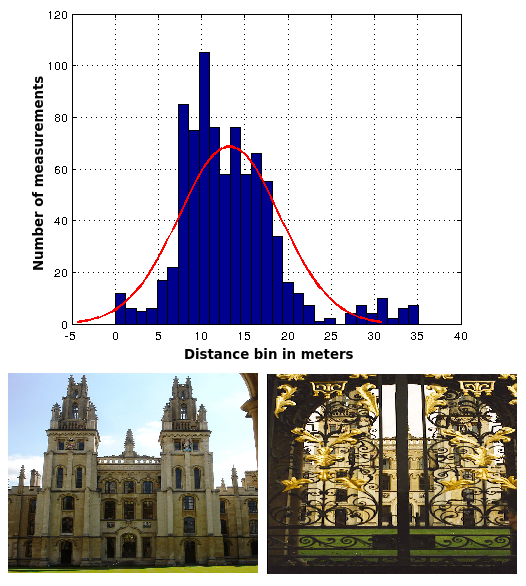
\includegraphics[width=11.0cm,height=12.0cm]{example_alias_occlusion_02}
\caption{Histogram of \gps localization error (top row) of a \emph{stationary} \gps sensor, showing
how inaccurate they can be. Bottom row is an example of two images belonging to the approximately same pose.
Visual localization is inaccurate here since in one image the object is occluded,
while \gps sensors give accurate localization.}
\label{fig:example_alias_occlusion_01}
\end{figure}
%%%%%%%%%%%%%%%%%%%%%%%%%%%%%%%%%%%%%%%%%%%%%%%%
There are several advantages and disadvantages of using \gps based localization
vis-a-vis visual localization approaches. Commercial viability of \gps sensors
make them \emph{cheap} to obtain, thus explaining their ubiquitousness. Such sensors are 
generally useful for obtaining coarse localization of objects in a \emph{global} coordinate
system. They are also not usually affected by the visual quality of an object's surroundings, 
\emph{i.e.} \gps sensors localize with similar accuracy irrespective of whether
they are used on a beach (no unique interest points) or near a popular monument (uniquely
identifiable structures), and they give \emph{unambiguous} localization to 
visually similar but differently located places.  However, \gps sensors are \emph{inaccurate} beyond a certain point, as
illustrated in Figure~\ref{fig:example_alias_occlusion_01}, and can fail in 
many environments due to reasons such as \emph{sporadic unavailability} of the satellite signal \cite{maier2010improved}. 
Thus, \emph{cheap, global, unambiguous, inaccurate, sporadic unavailability} are keywords
that characterize \gps sensors.

With the sudden increase of consumer cameras found on portable devices, vision based
localization approaches are also now \emph{cheaply} available. Such approaches are
generally useful for fine localization of objects in a \emph{local} coordinate
system relative to a reference frame. Compared to \gps sensors, vision based
localization systems also provide reasonable \emph{accurate} estimates of the
object's location. However, chances of \emph{ambiguities} are higher
in vision based localization methods since visual similarity of two
images of far apart places can lead to erroneous localization estimates. However,
since vision based localization methods are not dependent on satellite 
connectivity, such approaches are readily \emph{available} for utilization. Thus
vision based localization approaches can be characterized to be \emph{cheap, local,
ambiguous, accurate and available}. 

Notice that the two sensors have
complimentary advantages and disadvantages.
Thus, it is natural to ask {\em why not combine the advantages of both to 
improve their accuracy and reliability (Figure \ref{fig:flow_diag_concept_02})}. 
With recent portable devices carrying both \gps and vision based sensors, we
answer this increasingly important question in this paper.
In section~\ref{sec:related_work}, we discuss related work. We then describe
an approach to improve visual localization using \gps sensory output in
section~\ref{sec:gps_localization_feature}. Then we elaborate on an approach to 
improve \gps output using visual information in section~\ref{sec:improve_gps_img_retr}, before
describing an experiment that complimentarily fuses both the improved
estimates to do sequential localization in section~\ref{sec:improve_localization}.
Finally we performed the relevant experiments on collected dataset to demonstrate
the results of our approach in section~\ref{sec:experiments_results}, 
and conclude in section~\ref{sec:summary}.

%%%%%%% Block Diagram%%%%%%%%%%%%%%%%%%%%%%%%%%%%
\begin{figure}[t]
\centering
%\includegraphics[width=8.0cm,height=4.5cm]{block_diagram_01}
\subfloat[ ]{ 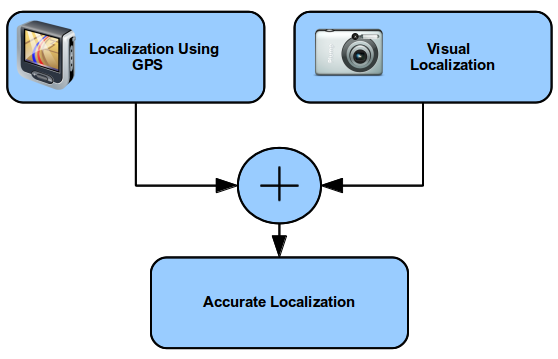
\includegraphics[width=9.0cm,height=7.0cm]{flow_diag_concept_02} \label{fig:flow_diag_concept_02}} \\
\subfloat[ ]{ 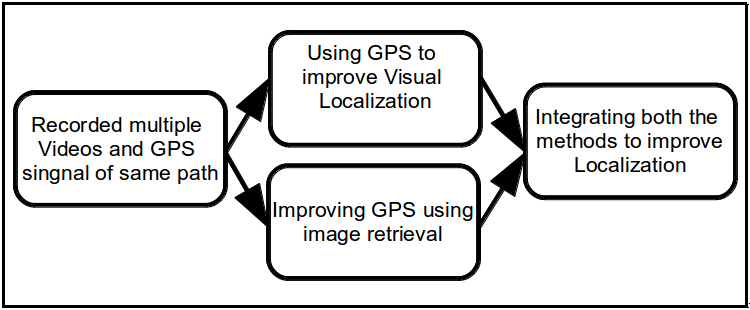
\includegraphics[width=8.0cm,height=3.0cm]{new_block_diagram} \label{fig:block_diagram}}
\caption{
(a) Problem Statement: We want to simultaneously use the 
noisy \gps signals and erroneous visual localization to 
generate accurate localization. (b) The block diagram of the proposed method.} 
\end{figure}
%%%%%%%%%%%%%%%%%%%%%%%%%%%%%%%%%%%%%%%%%%%%%%%% %%%%%%%%%%%%%%%%%%%%%%%%Flow Diagm%%%%%%%%%%%%%%

\subsection{Related Work}
\label{sec:related_work}

Unreliability in \gps tags critically affects many computer vision tasks
like 3D reconstruction and localization for shorter 
range \cite{lin2013cross,hafez2013visual}.
This unreliability in \gps has been addressed in several previous 
works\cite{hays2008im2gps}. This includes the use of
additional cues such as wifi strength \cite{martin2010precise}, additional special 
purpose hardware \cite{wei2011intelligent} or algorithms that learn error 
patterns \cite{cummins2008fab}. Vision based methods  have been used for 
\gps tag refinement. Most of the 
approaches often require a reference point (e.g. Street View) or dataset with
pre-assumed correct \gps tag in case of vision based refinement and 
multi sensor input in case of Kalman filter algorithms~\cite{maier2010improved}. 
Zamir {\em et. al.} \cite{Zamir_2014_CVPR}
propose a  self-refinement process,  that has an internal
noise reduction and robustness mechanism which effectively uses initial noisy 
\gps tags of the images to give refined values.
Accurate localization is critical to many robotic 
applications \cite{milford2012seqslam,cummins2011appearance}.

Visual localization is the problem where the location
of a query image is identified by comparison with location-tagged images
in a database. Its a challenging problem
because images of even the most common scenes like
urban environments show wide diversity in appearance. They can vary 
on different parameters e.g. different viewpoint, scale, occlusion, illumination etc. 
than the prior images in the database. For this paper we refer occlusion as blocking of 
the camera view because of non permanent objects. An occlusion in 
foreground (refer Figure \ref{fig:example_alias_occlusion_01}) or similar looking images 
for example, could degrade visual localization. Performance evaluation in visual localization is measured as the 
Euclidean distance between the \gps tags of query image and 
retrieved images \cite{milford2012seqslam}. Due to inaccuracies in \gps devices people integrate other sensor data like IMU, wheel odometry, and LIDAR sensors \cite{levinson2007map,wei2011intelligent} to get an accurate localization. 

\subsection{Contributions}
In this work we propose a method which localizes with an
accuracy of 7.5m by fusing vision and \gps together. 
In this regard, we address 3 main challenges in visual and \gps
localization: (i) \emph{Perceptual aliasing}, when similar-looking images
have very different \gps locations, (ii) \emph{camera occlusion}
(Figure~\ref{fig:example_alias_occlusion_01}), when dissimilar images
are co-located, and (iii) noisy \gps data. To do this, we present an approach to learn the useful feature \cite{turcot2009better,knopp2010avoiding} to improve the localization performance, along with an approach to correct noisy \gps outputs using visual localization~\cite{Zamir_2014_CVPR}.\\

\textbf{Dataset:} To do experiments in this paper, we collect
10 video datasets using a Contour action camera, while walking
along a 600m path repeatedly over 10 days. We extract images from
these videos at {\tt10fps} or {\tt1fps} depending on the requirement.
We then extract SIFT features and store them for each frame.
While processing one video, images from the other 9 are used to
build the visual bag of words vocabulary for image retrieval.

\section{Use of GPS for Better Visual Localization and Extracting Useful Features}
\label{sec:gps_localization_feature}
%\subsection{Visual Localization }
Visual localization problem is often formulated as an 
image retrieval problem. To achieve this visual features are extracted and 
clustered to form a visual vocabulary. Bag-of-Word model 
represents the image database as unordered set of visual 
words in the form of ``inverted index''. Inverted index is 
represented as a $(key,value)$ pair where key is the 
visual word index, and value is list of the images in which 
it appeared with their corresponding reliability weights. We 
identify the visual words in a query image using standard techniques \cite{nister2006scalable}.
With the help of visual words and inverted index score of $n^{th}$ retrieved image is computed as:
\begin{equation}
Score(img_n)= \sum_{z_k \in Z_q}W_k^n 
\label{eq:cal_score_query_img}
\end{equation} 
where $Z_q$ is the set of feature descriptors in query image 
and $W_k^n$ is the reliability weight of visual word corresponding 
to the $z_k$ feature descriptors in $n^{th}$ image. The image with 
highest score is chosen as the best matching image corresponding 
to the query image. Due to occlusion while extracting the features from an image many noisy
features are extracted. This includes features generated around 
unstable interest points. Noisy feature rejection is motivated by 
the fact that occlusion and unstable object features will be 
likely to exist in a single image, while useful features are 
likely to be found in multiple images of the same object or location. 
Identifying the features which are robust to change
in view can be determined by tracking which features exist in multiple 
views and are geometrically consistent with one another. 
This requires a minimum of two views, assuming that the object or location
exists in the database prior to the useful feature extraction stage.
%In order to do so 
%it requires minimum two views of a given object or location exist in
%the image database prior to useful feature extraction.\\

%%%%%% Original Features VS Useful Features %%%%%%%%%%%%%%
\begin{figure}[t]
\centering
\subfloat[ ]{ 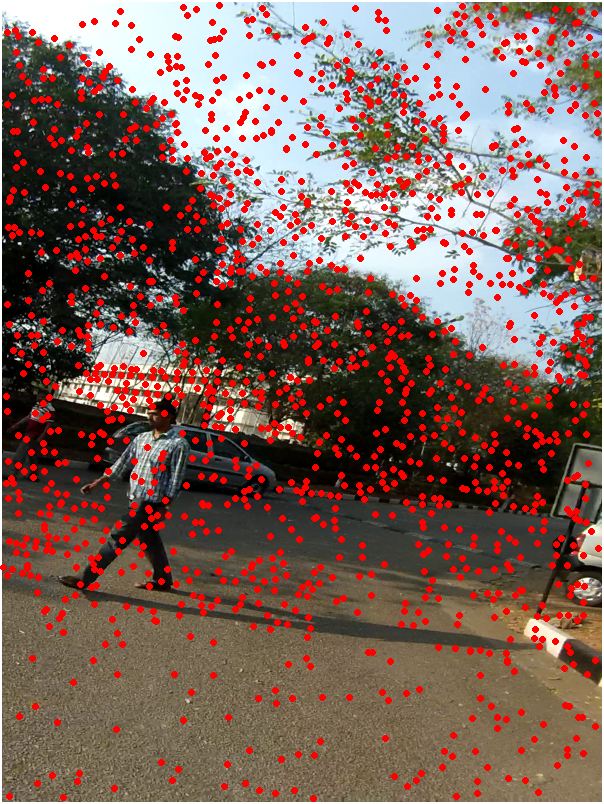
\includegraphics[width=6.0cm,height=8cm]{img_all_features_01}}
\subfloat[ ]{ 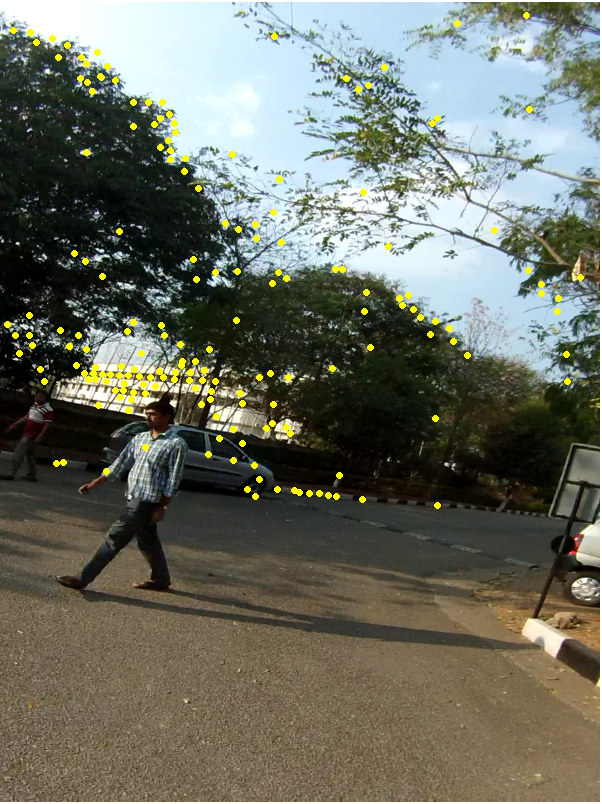
\includegraphics[width=6.0cm,height=8cm]{img_useful_features_01_yellow}}
\caption{Original image features (a) vs those features which could 
be considered useful features (b). Transient objects, occlusions in the 
foreground and non-distinctive areas of the scenes are found to 
be without useful features.}
\label{fig:all_feature_useful_feature}
\end{figure}
%%%%%%%%%%%%%%%%%%%%%%%%%%%%%%%%%% 

%%%%%% Flow Chart of Section 3 %%%%%%%%%%%%%%
\begin{figure}[h]
  \centering
  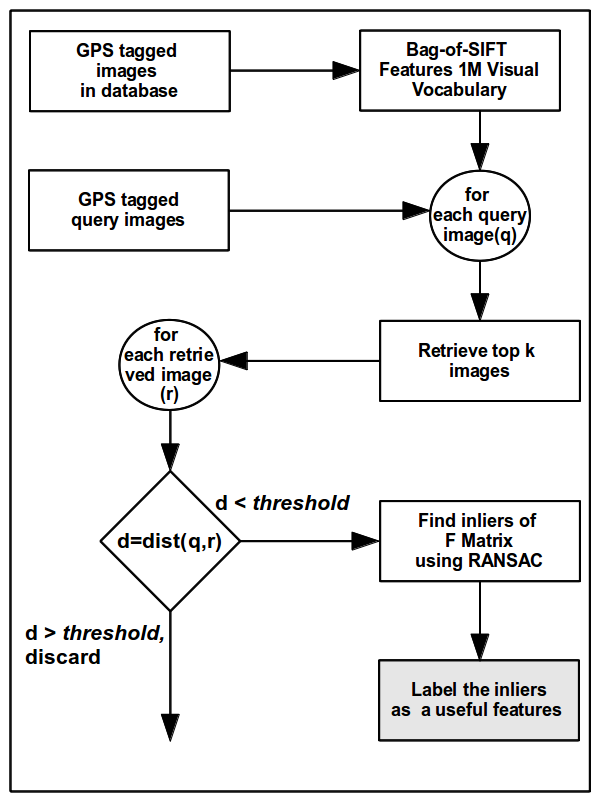
\includegraphics[width=10.0cm, height=11.5cm]{flow_diag_useful_features}
  \caption{ Flow chart to extract the useful features. For each query image we retrieve top k images using SIFT BoW. If the geographical distance between the query image and the retrieve image is less then a threshold then we find the inliers between tag them as a useful feature.}
  \label{fig:flow_diag_useful_features}
\end{figure}

%\subsection{Extracting the Useful Features and Role of GPS}
\textbf{Extracting Useful Features and Role of GPS:}
%%\label{sec:extract_use_features}
To determine the useful image features Bag-of-words of image 
database containing the full feature set is constructed. 
Each image in the database is used as a query 
and the top $k$ images are retrieved. All the images in the database have 
\gps tags associated with them. In order to avoid the perceptual aliasing 
and camera occlusion we considered only those images which lie in the radius 
of distance $d$ from the query image. Inliers are then used to estimate epipolar 
geometry and only features which are geometrically consistent  labeled as useful features. 
We perform experiments for $d$ = 10,20 and 30 meters and show how it effects
visual localization. For details of these experiments please refer sub-section \ref{subsec:useful_features_visual_localization}.
A sample result of useful feature extraction is shown in
Figure~\ref{fig:all_feature_useful_feature}.
Note that the image has more than 70\% non-distinctive area with occlusion. 
Our approach has filtered out almost all the noisy features generated around transient 
object and non-distinctive area. Figure \ref{fig:flow_diag_useful_features} 
describes the flow diagram of the proposed method.

\section{Improving GPS Signals through Image Retrieval}
\label{sec:improve_gps_img_retr}
Zamir {\em et. al.} \cite{Zamir_2014_CVPR} proposed a self refinement 
method to refine user-specified \gps tags of images. We extend their
work and apply it to discrete noisy \gps signals in order to get more accurate 
and consistence \gps signals, which we term refined \gps signals.
\subsection{Details of Algorithm}
\label{sec:detail_denosing_algo}
We have a set S = $ \{(V_1,G_1),(V_2,G_2),.. (V_n,G_n)\}$ where $V_i$ and $G_i$ is the $i^{th}$ 
video and it's corresponding \gps signal. Each \gps signal $G_i$ has a noise attached 
with them $G_i = \hat{G_i} + \eta$, where $\hat{G_i}$ is the refined signal and $\eta$ is the 
noise attached to $G_i$. Our goal is to extract out $\hat{G_i}$ in a self-refinement manner 
without using any external reference point.

We sample each \textit{V$_i$} at {\tt 1fps} and use each frame as query image $~\mathcal{I}$ 
against the rest of the frames from the set \{S-\textit{V$_i$}\}, and retrieve the top $\mu$ matches 
$\{m_1,m_2,.. m_\mu \}$ for each $~\mathcal{I}$. We use SIFT Bag-of-Words with vocabulary 
size of 1 million for the purpose of image retrieval. We then form  
$\bigl(\begin{smallmatrix}
\mu \\ 2\\
\end{smallmatrix} \bigr)$ 
triplets from each query image \& each pair of database images and estimate the relative location of
the triplet by using Bundler for camera localization~\cite{wu2011multicore}. For each triplet \{$~\mathcal{I}, m_i, m_j$\} 
we get \{$l_\mathcal{I}, l_i, l_j$\} which are camera locations of 
 $\mathcal{I},m_i,$ and $m_j$ in the SfM local co-ordinate system. 
However, we note that since in most images the relative height of the camera
w.r.t the ground is the same, we could transform these 3D vectors into 2D vectors. Thus, applying an assumption that video tracks were recorded 
roughly on a planar surface we can reduce the dimensionality of $l_\mathcal{I}, l_i$ and $l_j$ to two (e.g. using PCA).\\
Our aim is to calculate the \gps of $\mathcal{I}$ using the image triplet \{$l_\mathcal{I},
l_i, l_j$\}. To do this, the locations \{$l_\mathcal{I}, l_i, l_j$\} should be mapped from SfM local
co-ordinate system to the global \gps co-ordinate system. These two Cartesian co-ordinates are
related through a similarity transformation matrix $RST$.

\begin{equation}
\begin{bmatrix}
g\\
1\\
\end{bmatrix} = (\textbf{RST})
\begin{bmatrix}
l\\
1\\
\end{bmatrix}
\label{eq:mapping_g_l}
\end{equation}
where \textit{l} is a point in the SfM coordinate system and \textit{$g$} is it's corresponding point in global \gps co-ordinate system,
$\bigl[\begin{smallmatrix}
g\\ 1\\
\end{smallmatrix} \bigr]$
and 
$\bigl[\begin{smallmatrix}
l\\ 1\\
\end{smallmatrix} \bigr]$
are homogeneous co-ordinates of \textit{$g$} and \textit{$l$}. $RST$ is denoted by $3 \times 3$ matrix. 
We need at least two pairs of $g \leftrightarrow l$ correspondence in-order to calculate the $RST$ matrix from 
Equation \ref{eq:mapping_g_l}. In each triplet $m_i$ and $m_j$ are \gps tagged, we use their \gps tags 
and their locations $l_i$ and $l_j$ to compute $RST$ of the triplet. Now this transformation is used for finding the 
location of $\mathcal{I}$ in global \gps co-ordinate system. %Equation \ref{eq:conv_l_g}.
Since we have $\bigl(\begin{smallmatrix} \mu \\ 2\\ \end{smallmatrix} \bigr)$ possible triplets, we
  will get $\bigl(\begin{smallmatrix} \mu \\ 2\\ \end{smallmatrix} \bigr)$ possible \gps estimates for a query image.

\subsubsection{Robust Estimation through Random Walks}
The estimated \gps locations of $\mathcal{I}$ yielded by the triplets is accurate only if the \gps tag of reference images $m_i$ and $m_j$ is accurate. 
%However this is not the case with us since we are assuming that while recording there is noise in GPS signal hence it is very much possible that considerable number of
% triplet estimation are inaccurate. 
We use Random Walks on estimated triplets 
to discover the reliable subset of estimations. We define 
a graph $\mathcal{G}$ = (N,E) where N and E represent the 
set of node and edges. Each node represents one estimation, i.e. 
N = \{$g_1, g_2, ...g_\lambda$\}, and there is and edge between each 
pair of nodes, E = \{$(g_i , g_j ),i \neq j$ \}. We include the 
original \gps tag of $~\mathcal{I}$, for the estimation of its 
correct \gps-location, in set N. The transition probability from node $i$ to 
node $j$ according to their \gps distance is calculated using Equation 
\ref{eq:prob_nodes} given by Zamir {\em et. al.} \cite{Zamir_2014_CVPR}:

\begin{equation}
p(i,j)=\frac{e^{-\sigma||g_i-g_j||_2}}{\sum_{k=1}^{\lambda} e^{-\sigma||g_i-g_k||_2} }
\label{eq:prob_nodes}
\end{equation}
where $||.||_2$ denotes the $l_2$ norm, $\lambda$ is the number of node in 
graph $\mathcal{G}$ and $\sigma$ is call insensitive parameter.
%Equation \ref{eq:prob_nodes} models the fact that closer the point more consistence they are and higher the transition probability for those pair of nodes, value of $\sigma$ is set to .0005. The denominator act as a normalizer, it normalize the summation of the transition probability from a node to all other nodes.

\textbf{Image Geo Density and Initial Node Score:}
The purpose of image geo density is to handle the phenomenon
of non uniform distribution of images across popular sites
like flickr, facebook, etc \ldots
% , example 
% images from the social media like flickr, facebook etc. images 
% related to the popular
% sites will be more in number as compare to the unpopular.
% Hence in the image retrieval the images from popular sites
% are more likely to be retrieved as compare to unpopular one.
% In these circumstances \cite{Zamir_2014_CVPR} geo-densities is the 
% deciding factor for the initial score of nodes. 
In our case, where we have multiple videos of the same path, we can 
assume uniform distribution of images. The initial score
of the nodes is not going to be effected by geo-density, hence
initial score of the $n^{th}$ node $v(n)$ can be calculated as:

\begin{equation}
v(n)=\frac{1}{\lambda }
\end{equation}

\subsubsection{Adaptive Damping Factor}
For a each query image we got a graph $\mathcal{G}$ having $\lambda$ nodes where 
each node is initialized with score $v(n)$.
The Random Walks algorithm will update the score of one node at every iteration using the transition probability from other nodes to it. Equation \ref{eq:basic_random_walk} is the basic Random Walks formula 
\begin{equation}
x_{(k+1)}(j) = \sum_{k=1}^{\lambda} \overbrace{\alpha}^{\text{\textcircled{1}}} x_k(i)p(i,j) + \overbrace{(1-\alpha)}^{\text{\textcircled{2}}}v(j)
\label{eq:basic_random_walk}
\end{equation}    
where $x_k$(i) is the relevance score of $i^{th}$ node at $k^{th}$ iteration. 
%The argument of summation is part computes the probability of transition from all nodes to single particular node, and the right one is a damping term. 
The use of the damping term in Random Walks is to use the prior knowledge about the relevance of nodes and to ensure irreducibility of 
the transition probabilities matrix which is a convergence condition for Random Walks ~\cite{jing2008visualrank}. 
The summation of term \textcircled{1} and term \textcircled{2} in Equation \ref{eq:basic_random_walk} should be 1 
because the relevance score at any iteration must sum to one, \emph{i.e.},
$\sum_{k=1}^{\lambda}x_k(i)=1$. Zamir et al. \cite{Zamir_2014_CVPR} further propose an adaptive
damping factor which adaptively changes according to the consistency of each node w.r.t others. They
formulate the damping term of a node as a function of its relevance score at each iteration:
\begin{flalign}
x_{k+1}(j)  =  \frac{1}{\eta}\Big(\sum_{i=1}^{\lambda} \overbrace{\big(1-(1-\alpha \big)x_{k}(j))}^{\text{\textcircled{1}}}x_k(i)p(i,j)    \nonumber\\ +   \overbrace{(1-\alpha)x_k(j)}^{\text{\textcircled{2}}}v(j)\Big)
\label{eq:damping_factor_random_walk}
\end{flalign}

%The difference between Equation \ref{eq:damping_factor_random_walk} and \ref{eq:basic_random_walk} is of damping term in Equation \ref{eq:damping_factor_random_walk} the damping term \textcircled{2}. 
%The amount of contribution of a node from it's initial score also depends its so-far consistency with all other nodes. The damping term stops the propagation of random noise to the output. 
The normalization constant $\eta$ given by Equation \ref{eq:norm_constant_random_walks} forces the
sum of all relevance scores to be one.

\begin{flalign}
\eta  =  \sum_{j=1}^{\lambda} \Big(\sum_{i=1}^{\lambda} \big(1-(1-\alpha \big)x_{k}(j))x_k(i)p(i,j)    \nonumber\\ +   (1-\alpha)x_k(j)v(j)\Big)
\label{eq:norm_constant_random_walks}
\end{flalign}

\textbf{Estimation of Final GPS-Tag using the Relevance Scores:}
The estimations which are badly effected by noise are expected to have relevance score of $\approx$ 0, other nodes should gain the score based on their transition probability and initial score. Finally we compute the refined \gps-tags of the query $~\mathcal{I}$, utilizing a weighted mean using the relevance scores $x_\pi$. 
\begin{equation}
\hat{g} =  \sum_{i=1}^{\lambda}g_ix_\pi(i)
\end{equation}
where $\hat{g}$ is refined \gps-tags.

\section{Improving the Localization}
\label{sec:improve_localization}
\textbf{Integrating Visual Localization and GPS Refinement:} 
In section \ref{sec:gps_localization_feature} we have shown 
how with the help of \gps we can 
overcome issues like occlusion and perceptual aliasing 
in order to improve visual localization using image retrieval,
whereas section \ref{sec:improve_gps_img_retr} describe how to reduce the error in \gps
signal with the help of image retrieval and random walks. As mentioned
above, we integrate both modules to improve localization 
in challenging scenarios like over short distances where \gps signals tend to fail.
First we improve \gps signals and label all the images in the database with 
refined \gps tags. 
Using these refined \gps tags we filter out the useful
features for building a vocabulary and inverted index.

\textbf{Sequential Localization:} Without any loss of generality, we can assume 
that the motion of any portable device with \gps is a smooth motion. So we 
can assume such motion satisfies the
Markov assumption {\em i.e.} that is the current pose $X_t$ is dependent only on
the previous pose $X_{t-1}$. Our sequential visual localization method consists 
two phases: initial localization phase and query retrieval phase.
In initial localization phase we keep on retrieving relevant images to the query image  
until estimation of the pose is known to us with minimum probability $P^*$.
$P^*$ is calculated using Algorithm \ref{algo:estimation_init_prob}.
Once the initial pose $X_t$ is fixed we use temporal sequence property 
to fix the pose of $X_{t+1}$ in query retrieval phase. 
In section 5 we have demonstrated the effect of useful features, refined signal as well as 
combined effect of both on localization by conducting different set of experiments.
We also performed the sequential localization after integration.


%%%%%%%%%%%%%%%%%%%%%%%%%% THE ALGORITHM%%%%%%%%%%%%%%%%%%%%%%%%%%%%%%%
\alglanguage{pseudocode}
\begin{algorithm}[h]
\caption{Estimation of initial pose}
\label{algo:estimation_init_prob}
\begin{algorithmic}[1]
\State \textbf{Input:} Bag-of-Word frame work, $Q$: Queue
\State \textbf{Output:} Initial pose with minimum probability $P^*$.
%%\State Re-sampled the Query video at $1fps$ and Training Videos at $5fps$.
\For{i=1 $\rightarrow$ $N$} 
	\State $r_i$ $\leftarrow$ Retrieved image using query image $q_i$.
	\If{$Q$ is NULL}
		\State $Q$ $\leftarrow$ $r_i$
	\Else
		\For{j=1 $\rightarrow$ Number of element in $Q$} 
		 	\State $dist$ = calEculideanDistance($r_i$,$Q_j$)
			\If {$dist < thresholdDistance$ }
 				\State Score($Q_j$) = Score($Q_j$) + 1
 			\Else
 				\State $Q$ $\leftarrow$ $r_i$
	 		\EndIf
		\EndFor
	\EndIf	
\EndFor
\State $P^*$ = arg max(Score($p_k$) / N ; where $p_k$ $\in$ Q
\State Return the pose corresponding to $p_k$
\end{algorithmic}
\end{algorithm}
%%%%%%%%%%%%%%%%%%%%%%%%%%%%%%%%%%%%%%%%%%%%%%%%%%%%%%%%%%%%%%%%%%%%%

\section{Experiments and Results}
\label{sec:experiments_results}

In this section, we demonstrate the utility of our approach with quantitative
experiments. 
We capture the videos using a Contour action camera \cite{contour_camera} with 
resolution $1920\times1080$ at $30fps$. The device also has an
inbuilt \gps sensor which recorded the corresponding \gps signal at $1Hz$.
This gives us two different loosely aligned signals \gps and videos. 
Since we are also interested in studying the utility of multiple runs
captured over time, we collect the videos on ten different days by walking on 
the same $600m$ long path. Data is captured in the evening at peak traffic hours to ensure 
approximately same crowded urban environment setting. This process yields ten videos
of the same path with labelled \gps tags.

For vision based localization, we use bag of words representation
with 1 M visual words built on top of dense SIFT descriptors. During all the experiments, we have ensured that
the test data is not used for the vocabulary construction. Wherever,
multiple runs are used, one run is used for the evaluation in the leave  one
out manner.

As can be seen in Figure~\ref{fig:noisy_refined_plot}, our sensor fusion scheme is
yielding superior estimates of the localization. One may notice the noisy (zig zag)
path of the original localizations and the more or less smooth path estimated 
after the multi sensor localization as we discussed in the previous section.
In the rest of this section, we demonstrate the quantitative results of various
experiments.
\begin{figure}[t]
\centering
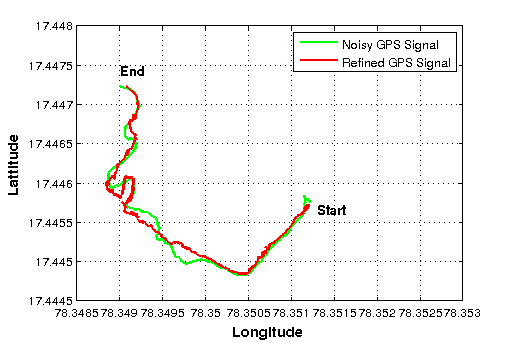
\includegraphics[width=11.0cm,height=9.0cm]{noisy_refined_plot}
\caption{Plot demonstrating the noisy and refined \gps signals. One can observe
refined \gps signal (red) is less random and in zig-zag shape as 
compare to noisy \gps signal (green).
}
\label{fig:noisy_refined_plot}
\end{figure}

%%%%%%%%%%%%%%%%%%%%%%%%%%%%%%%%%%
\subsection{Effect of Useful Features on Visual Localization}
\label{subsec:useful_features_visual_localization}
%We re-sampled the videos at $10 fps$. Using SIFT features 
%we build Bag-of-Word frame work with 1 million 
%visual vocabulary. Using each image as a query 
%we labelled the useful features for all the images.
First, we demonstrate the utility of feature selection in improving
the accuracy of localization.
Effect of useful features on visual localization performance was 
evaluated using K-fold cross validation with number of folds set to 10.
For each of the query image we retrieved an image 
from Bag-of-Words model build by using useful features only. 
If the Euclidean distance between retrieved image and 
query image is greater than $\delta_d$ distance 
it is consider as ``invalid localization''. The percentage error in the 
visual localization is define as:
\begin{equation}
P_e = \big( \frac{Total No. Of Invalid Localization}{No. Of Query Frames} \big) \times 100 
\label{eq:per_error_visual_localization}
\end{equation}
In this experiment we have set the $\delta_d=10m$. Table~\ref{table:useful_feature_comparison} shows 
the comparative percentage error in visual localization between two approaches. 
%{\bf Add 2-3 sentences on (i) What should be exactly noticed in this table.
%(ii) What is OF? What is UF? (iii) Which colums should be compared which rows should be
%compared?}
In the table experiment $E_i$ means $i^{th}$ video is used as 
the source for query images and rest all are use in building visual vocabulary.
One can observe significant drop in error while using useful
features for visual localization.
\begin{table}[t]
\centering
\caption{Effect of useful features on visual localization. There is a 
significant drop in percentage error in visual localization with useful features.
As $d$ increases the increase in number of inliers are very less. Therefore useful 
features are almost constant for different values of $d$. Hence the drop 
in $P_e$ error is less. NA=Not Applicable, OF=Original Features, UF=Useful Features as shown in 
Figure \ref{fig:all_feature_useful_feature}.}
 %\resizebox{.45\textwidth}{.11\textwidth} { \begin{tabular}{|c|c|c|c|c|}
\begin{tabular}{|c|c|c|c|c|}
\hline

   Exp. &  \textit{$P_e$, d=NA} & \textit{$P_e$, d=10} & \textit{$P_e$, d=20} & \textit{$P_e$,
   d=30}\\  %\cline{2-5}
   No.~ & \textit{OF} & \textit{UF} & \textit{UF} & \textit{UF} \\ \hline
    $E_1$ & 31.63 & 23.56  & 22.69 & 22.57 \\ \hline
    $E_2$ & 31.70 & 23.47  & 22.65 & 22.59 \\ \hline
    $E_3$ & 29.49 & 22.21  & 21.49 & 21.52 \\ \hline
    $E_4$ & 32.06 & 23.93  & 23.03 & 22.98 \\ \hline
    $E_5$ & 30.54 & 22.89  & 22.15 & 22.15 \\ \hline
    $E_6$ & 31.98 & 23.07  & 22.26 & 22.23 \\ \hline
    $E_7$ & 31.04 & 22.87  & 22.15 & 22.09 \\ \hline
    $E_8$ & 30.68 & 22.72  & 22.13 & 22.07 \\ \hline
    $E_9$ & 31.75 & 23.47  & 22.70 & 22.58 \\ \hline
    $E_{10}$ & 32.30 & 23.72  & 22.63 & 22.56 \\ \hline
    \end{tabular}
\label{table:useful_feature_comparison}
\end{table}
The other observation that can be made is, the drop in percentage error $P_e$ 
is less for increasing 
values of $d$. It is because of 
number of inliers are almost constant with varying $d$.
Hence we set $d=10m$ for further experiments to expedite 
the process without compromising accuracy a lot. 
%{\bf What should be the take home message of this experiment?}

\subsection{Refined vs Noisy GPS Signals RMSE Score}
The recorded GPS signal has noise associated with it. To motivate, if one log the
\gps signal while keeping the device stationary, one can see  large
variation in \gps values up to 35m (as shown in Figure \ref{fig:example_alias_occlusion_01}). 
The term noisy \gps signals refer to the \gps signals 
which were recorded using \gps receiver. By improving the
\gps signals using images (section \ref{sec:improve_gps_img_retr}) we get refined \gps signals.

To refine a \gps signal the corresponding video run was used 
as the query video in the vision based localization. We do this for
each of the videos separately.
Using all these attempts, we refine the 
\gps tags and finally we integrate all the {\sc gps} tags to
get the refined \gps signal.

 To quantitatively compare, we used Root Mean Square
Estimate(RMSE) values. We assumed one of the \gps signal 
as a ground truth and calculated the RMSE for other signals with respect
to assumed ground truth. RMSE for the $G_n$ \gps signal is given as:
\begin{equation}
RMSE(G_n) = \frac{ \sqrt[2] {\sum_{i=0}^{N} \Big( \textit{Dist}(G_{gt}(i),G_n(i)) \Big )^2 } } {N}
\end{equation}
where  $ N = \min \big( length(G_{gt}),length(G_n) \big) $ as all the signals are approximately same
length, so discarding few values will not effect the RMSE much,  $G_{gt}(i)$ and $G_n(i)$ is
$i^{th}$ \gps reading of assumed ground truth signal and $n^{th}$ \gps signal
respectively. \textit{Dist} calculates the Euclidean distance between two \gps measurements. Mean
RMSE of the $n^{th}$ \gps signal is the mean of all the RMSE values taking $n^{th}$ signal as a
ground truth. We calculated RMSE values for noisy \gps signals and refined \gps signals
separately. Table \ref{table:rmse_mean_err_comparison} shows the comparison between Mean RMSE values
of noisy and refined \gps signals for each video.   $S_n$ indicates that $n^{th}$ signal was taken as 
ground truth to calculate the Mean RMSE. The Mean RMSE for the noisy \gps signal is $\approx$10m 
whereas for refined \gps signals it comes down to $\approx$6-7m. This demonstrates that the sensor fusion is resulting in a more consistent localization results than using a single sensor alone.

\begin{table}[h]
\centering
\caption{Mean RMSE comparison of noisy and refined \gps signal. For refined
\gps signal RMSE values $\approx$7m.}
	\begin{tabular}{|c|c|c|c|}
  %\resizebox{.42\textwidth}{.088\textwidth} {\begin{tabular}{|c|c|c|c|}
\hline
   \textit{Run No.} & \textit{RMSE } & \textit{RMSE } & \textit{\% drop in}\\ 
    ~ & \textit{Noisy Signal} & \textit{Refined Signal} & \textit{RMSE Error} \\ \hline
    $S_1$ & 9.81 & 6.76  & \textbf{31.10} \\ \hline
    $S_2$ & 10.55 & 7.36 & \textbf{30.23} \\ \hline
    $S_3$ & 10.49 & 7.01 & \textbf{33.17} \\ \hline
    $S_4$ & 9.76 & 6.73  & \textbf{31.05} \\ \hline
    $S_5$ & 9.54 & 6.79  & \textbf{28.82} \\ \hline
    $S_6$ & 10.31 & 6.98 & \textbf{32.30} \\ \hline
    $S_7$ & 10.21 & 6.92  & \textbf{32.22} \\ \hline
    $S_8$ & 10.01 & 6.87  & \textbf{31.36} \\ \hline
    $S_9$ & 10.65 & 7.01  & \textbf{34.17} \\ \hline
    $S_{10}$ & 9.96 & 6.95  & \textbf{30.22} \\ \hline
    \end{tabular}
\label{table:rmse_mean_err_comparison}
\end{table}

\subsection{Comparison of Denoising using Synthetic Noise}
In another experiment to test the method in various extreme circumstances 
we added random Gaussian noise as an input error with mean values 100, 500, 1000, 2000, 
3000 and 4000 meters to 5, 10, 20, 33 and 50 percent of the 24648 images in 
our dataset and the standard deviation was set to the half the mean to 
replicate the \gps device error with $mean = 12.23m$ and 
$standard$ $deviation$ = $5.98$ (Figure \ref{fig:example_alias_occlusion_01}). 
We improvised the synthetic error on the top of the already existing noise. 
Hence, the additional synthetic noise determines the lower bound of 
noise since the exact amount of error in the dataset is unknown. 
We also made sure that in this experiment, the query images were among
the ones with contaminated \gps tags to ensure the evaluation fair and challenging. 
We got similar results like Zamir {\em et. al.} \cite{Zamir_2014_CVPR}(Figure \ref{fig:synthetic_noise}). We observed  for the contamination percentages less 
than 33\%, the method almost completely eliminates the error 
regardless of the mean of the contamination in the input. 
Once the input error increase beyond the 33\% and 50\% the
error in output is no more avoidable yet still less than the error in input.

\begin{figure}
\centering
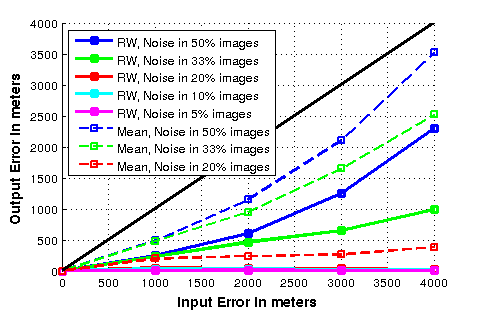
\includegraphics[width=11.0cm,height=9.0cm]{synthetic_noise}
\caption{Plot is demonstrating the synthetic noise reduction process and comparison between Random walks and simply taking the mean. It is clear from the graph as contamination percentage increase Mean is not that much efficient comparison to Random walks in order to remove the added noise.
}
\label{fig:synthetic_noise}
\end{figure}

\begin{table}[h]
\centering
%%\small
\caption{Effect of refined signal on percentage error. With small value 
of $\delta_d$ there is significant difference in the performance. As 
$\delta_d$ increases the performance gap is narrowed down.NS = Noisy Signal, RS = Refined Signal.}
	\begin{tabular}{|c|c|c|c|c|c|c|}
\hline
\textit{Exp.No.}& \multicolumn{2}{c}{$P_e$, $\delta_d$=7.5m} & \multicolumn{2}{c}{$P_e$, $\delta_d$=10m} & \multicolumn{2}{c|}{$P_e$, $\delta_d$=15m} \\ \hline
 ~  & NS  & RS & NS  & RS & NS  & RS \\ \hline
 $E_1$ & 45.98 & 29.68 & 31.63 & 23.11 &  16.05 & 15.33 \\ \hline
 $E_2$ & 40.00 & 33.68 & 31.73 & 30.73 &  18.53 & 20.00 \\ \hline
 $E_3$ & 32.00 & 27.85 & 24.09 & 24.52 &  16.19 & 14.28 \\ \hline
 $E_4$ & 33.00 & 24.50 & 25.24 & 21.28 &  13.61 & 10.00 \\ \hline
 $E_5$ & 37.12 & 29.09 & 29.43 & 22.19 &  16.30 & 14.80 \\ \hline
 $E_6$ & 39.00 & 28.67 & 28.84 & 25.05 &  17.46 & 15.09 \\ \hline
 $E_7$ & 38.85 & 28.72 & 28.19 & 24.23 &  16.57 & 14.91 \\ \hline
 $E_8$ & 37.18 & 28.99 & 27.79 & 25.45 &  16.47 & 15.00 \\ \hline
 $E_9$ & 40.49 & 29.81 & 30.35 & 23.52 &  15.82 & 14.73 \\ \hline
 $E_{10}$ & 36.72 & 30.01 & 28.80 & 24.74 &  16.14 & 14.94 \\ \hline
\end{tabular}
\label{table:localization_refined_signal}
\end{table} 

\subsection{Effect of Refined GPS Signal On Localization:}
We also performed the experiments to study the effect of refined \gps signal on localization. The ten videos sampled at $10fps$ and tagged each frame with their corresponding noisy and refined \gps tags. 
Bag-of-Word framework was build using SIFT features from the nine runs with 
visual vocabulary set to 1 million words. We performed visual localization using 
one of the video run as a query dataset. Percentage error in visual localization 
for distance was calculated
using Equation \ref{eq:per_error_visual_localization}. Table \ref{table:localization_refined_signal} shows the 
comparison in visual localization performance between refined and noisy \gps 
signal for different $\delta_d$ distances. An experiment $E_i$ means $i^{th}$ run was used as a query run(different query run contains 4000-4193 frames) and rest all other for vocabulary building. From the Table \ref{table:localization_refined_signal} 
one can also infer that for $\delta_d$ = 7.5m the difference in the $P_e$ error for noisy \gps signal and refined signal is huge, but as $\delta_d$ increases from 10m and beyond $P_e$ is approximately same for both kind of signals. Variance in the $P_e$ for refined \gps signal 
less than noisy \gps signal as standard deviation are 9.67 and 6.70 respectively 
for the noisy and refined signal.

\subsection{Multi Sensor Localization}
We integrated both the modules {\em i) Use of \gps for Better Visual Localization} and 
{\em ii)Improving the \gps Signal Through Image Retrieval} 
to form a pipeline for more accurate 
localization. First we refined the \gps signals using images and
adjusted the \gps tags therein to the correct locations.
Then we improved the visual localization by labeling the useful 
features with the help of refined \gps. 
The pipeline was tested on ten video runs, where each runs contains
4000-4193 frames. Nine runs were used to build the Bag-of-Word frame 
work for image retrieval having vocabulary size of 1 million visual words.
All the frames from a video run were used as query dataset. Percentage 
error in visual localization was calculated by the 
Equation \ref{eq:per_error_visual_localization}. We localize for the 
distance $\delta_d$ = 7.5m. We also performed the sequential localization
by fixing the initial position with Algorithm \ref{algo:estimation_init_prob}.
In the Algorithm \ref{algo:estimation_init_prob} we set N = 10($i.e$ re-sampling 
frequency of the videos) and $thresholdDistance$ = $\delta_d$ and $P^*$=0.7. 
Table~\ref{table:per_err_integrated_bow} and Figure \ref{fig:localization_comp} shows significant drop in $P_e$ with multi sensor localization method.
Our proposed method is useful to perform localization for a shorter distance($\approx 7.5m$) 
by fusing images and noisy \gps tags obtained by using any commercial \gps receiver. 

\begin{table}[h]
%%\small
\centering
\caption{Comparison of percentage error $P_e$ in localization with $\delta_d$ =7.5m while using the methods i)Bag-of-Words frame work ii)Bag-of-Words frame work + Integration of modules iii)Bag-of-Words frame work + Integration of modules + Sequential Localization.}
\begin{tabular}{|c|c|c|c|}
\hline
\textit{Exp.} & \textit{Simple} & \textit{BOW} & \textit{BOW Seq.} \\
No. & \textit{BOW} & \textit{Integration} & \textit{Localization} \\ \hline
	$E_1$ & 31.63 & 8.09  & 2.97 \\ \hline
	$E_2$ & 31.70 & 8.03 &  2.73 \\ \hline
	$E_3$ & 29.49 & 7.10 &  2.14 \\ \hline
	$E_4$ & 32.06 & 10.03 & 3.30 \\ \hline
	$E_5$ & 30.54 & 7.60 &  2.71 \\ \hline
	$E_6$ & 31.98 & 9.07 &  2.85  \\ \hline
	$E_7$ & 31.04 & 8.10 &  2.56 \\ \hline	
	$E_8$ & 30.68 & 7.71 &  2.60 \\ \hline
	$E_9$ & 31.80 & 8.29 &  2.12 \\ \hline
	$E_{10}$ & 31.44 & 8.56 &  2.82 \\ \hline
\end{tabular}
\label{table:per_err_integrated_bow}
\end{table}
\newpage

\section{Summary}
\label{sec:summary}
This work proposed a multi sensor based localization scheme that  fuse two 
popular localization schemes to result in a more accurate localization strategy.
The objective of our work has been to fuse \gps signals and images together 
in order to improve the localization. We propose methods that use noisy \gps to
improve the vision based localization. We also propose methods that use vision based
localization to improve the \gps signals. Finally we use these two steps in an iterative
manner to get further improvement.
We also presented a set of experiments to validate the fusion schemes and thereby the
improvements in localization by fusing image and \gps.

\begin{figure}[t]
\centering
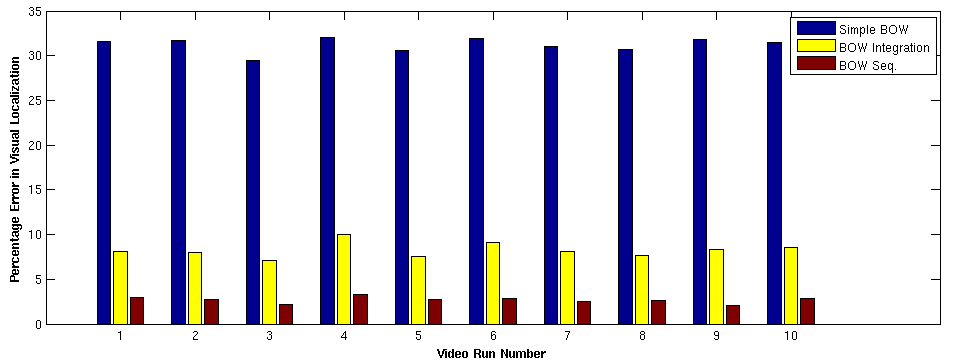
\includegraphics[width=\textwidth,height=8.0cm]{localization_comp.png}
\caption{Bar graph visualization of percentage error in localization using different methodologies.}
\label{fig:localization_comp}
\end{figure}